% Options for packages loaded elsewhere
\PassOptionsToPackage{unicode}{hyperref}
\PassOptionsToPackage{hyphens}{url}
%
\documentclass[
]{article}
\title{Report on Education 5W data -- Venezuela}
\author{Sean Ng}
\date{10 November, 2021}

\usepackage{amsmath,amssymb}
\usepackage{lmodern}
\usepackage{iftex}
\ifPDFTeX
  \usepackage[T1]{fontenc}
  \usepackage[utf8]{inputenc}
  \usepackage{textcomp} % provide euro and other symbols
\else % if luatex or xetex
  \usepackage{unicode-math}
  \defaultfontfeatures{Scale=MatchLowercase}
  \defaultfontfeatures[\rmfamily]{Ligatures=TeX,Scale=1}
\fi
% Use upquote if available, for straight quotes in verbatim environments
\IfFileExists{upquote.sty}{\usepackage{upquote}}{}
\IfFileExists{microtype.sty}{% use microtype if available
  \usepackage[]{microtype}
  \UseMicrotypeSet[protrusion]{basicmath} % disable protrusion for tt fonts
}{}
\makeatletter
\@ifundefined{KOMAClassName}{% if non-KOMA class
  \IfFileExists{parskip.sty}{%
    \usepackage{parskip}
  }{% else
    \setlength{\parindent}{0pt}
    \setlength{\parskip}{6pt plus 2pt minus 1pt}}
}{% if KOMA class
  \KOMAoptions{parskip=half}}
\makeatother
\usepackage{xcolor}
\IfFileExists{xurl.sty}{\usepackage{xurl}}{} % add URL line breaks if available
\IfFileExists{bookmark.sty}{\usepackage{bookmark}}{\usepackage{hyperref}}
\hypersetup{
  pdftitle={Report on Education 5W data -- Venezuela},
  pdfauthor={Sean Ng},
  hidelinks,
  pdfcreator={LaTeX via pandoc}}
\urlstyle{same} % disable monospaced font for URLs
\usepackage[margin=1in]{geometry}
\usepackage{longtable,booktabs,array}
\usepackage{calc} % for calculating minipage widths
% Correct order of tables after \paragraph or \subparagraph
\usepackage{etoolbox}
\makeatletter
\patchcmd\longtable{\par}{\if@noskipsec\mbox{}\fi\par}{}{}
\makeatother
% Allow footnotes in longtable head/foot
\IfFileExists{footnotehyper.sty}{\usepackage{footnotehyper}}{\usepackage{footnote}}
\makesavenoteenv{longtable}
\usepackage{graphicx}
\makeatletter
\def\maxwidth{\ifdim\Gin@nat@width>\linewidth\linewidth\else\Gin@nat@width\fi}
\def\maxheight{\ifdim\Gin@nat@height>\textheight\textheight\else\Gin@nat@height\fi}
\makeatother
% Scale images if necessary, so that they will not overflow the page
% margins by default, and it is still possible to overwrite the defaults
% using explicit options in \includegraphics[width, height, ...]{}
\setkeys{Gin}{width=\maxwidth,height=\maxheight,keepaspectratio}
% Set default figure placement to htbp
\makeatletter
\def\fps@figure{htbp}
\makeatother
\setlength{\emergencystretch}{3em} % prevent overfull lines
\providecommand{\tightlist}{%
  \setlength{\itemsep}{0pt}\setlength{\parskip}{0pt}}
\setcounter{secnumdepth}{-\maxdimen} % remove section numbering
\usepackage{booktabs}
\usepackage{longtable}
\usepackage{array}
\usepackage{multirow}
\usepackage{wrapfig}
\usepackage{float}
\usepackage{colortbl}
\usepackage{pdflscape}
\usepackage{tabu}
\usepackage{threeparttable}
\usepackage{threeparttablex}
\usepackage[normalem]{ulem}
\usepackage{makecell}
\usepackage{xcolor}
\ifLuaTeX
  \usepackage{selnolig}  % disable illegal ligatures
\fi

\begin{document}
\maketitle

\begin{quote}
This demo is an entirely automated report -- all charts and tables, as
well as all figures within the text have been generated from the data,
with no manual input. This report makes use of the outputs generated by
\texttt{5W\_cleaning.Rmd}, which automates the cleaning of 5W data. The
5W data used has had partner information removed.
\end{quote}

\hypertarget{summary-of-beneficiaries-by-activity-with-sex-ratio}{%
\section{Summary of beneficiaries by activity, with sex
ratio}\label{summary-of-beneficiaries-by-activity-with-sex-ratio}}

\begin{longtable}[]{@{}
  >{\centering\arraybackslash}p{(\columnwidth - 10\tabcolsep) * \real{0.65}}
  >{\centering\arraybackslash}p{(\columnwidth - 10\tabcolsep) * \real{0.06}}
  >{\centering\arraybackslash}p{(\columnwidth - 10\tabcolsep) * \real{0.11}}
  >{\centering\arraybackslash}p{(\columnwidth - 10\tabcolsep) * \real{0.06}}
  >{\centering\arraybackslash}p{(\columnwidth - 10\tabcolsep) * \real{0.06}}
  >{\centering\arraybackslash}p{(\columnwidth - 10\tabcolsep) * \real{0.07}}@{}}
\toprule
\begin{minipage}[b]{\linewidth}\centering
actividad
\end{minipage} & \begin{minipage}[b]{\linewidth}\centering
total
\end{minipage} & \begin{minipage}[b]{\linewidth}\centering
percent\_of\_total
\end{minipage} & \begin{minipage}[b]{\linewidth}\centering
male
\end{minipage} & \begin{minipage}[b]{\linewidth}\centering
female
\end{minipage} & \begin{minipage}[b]{\linewidth}\centering
sex\_ratio
\end{minipage} \\
\midrule
\endhead
DISTRIBUCION DE KITS DE MATERIALES ESCOLARES & 471,568 & 44.01 & 232,197
& 239,372 & 0.97 \\
ALIMENTACION ESCOLAR & 156,926 & 14.64 & 72,139 & 84,787 & 0.85 \\
PROMOCION MENSAJES CLAVES PARA LA COMUNIDAD ESCOLAR & 144,775 & 13.51 &
64,029 & 80,502 & 0.8 \\
EDUCACION A DISTANCIA & 132,258 & 12.34 & 64,240 & 68,018 & 0.94 \\
APOYO PSICOEDUCATIVO PARA NNA & 120,887 & 11.28 & 54,859 & 66,028 &
0.83 \\
FORMACION DOCENTE Y OTRO PERSONAL EDUCATIVO & 17,238 & 1.61 & 3,470 &
13,224 & 0.26 \\
ACTIVIDADES CON ADOLESCENTES Y JOVENES DE NIVELACION, HABILIDADES PARA
LA VIDA Y CAPACITACION TECNICA & 14,016 & 1.31 & 6,336 & 7,680 & 0.82 \\
BECAS Y OTROS INCENTIVOS PARA DOCENTES Y PERSONAL & 5,744 & 0.54 & 1,572
& 4,172 & 0.38 \\
ACTIVIDADES RECREATIVAS & 4,317 & 0.4 & 1,998 & 2,319 & 0.86 \\
INICIATIVAS PARA REINSERCION EDUCATIVA DE NNA FUERA DE LA ESCUELA &
3,869 & 0.36 & 2,114 & 1,755 & 1.2 \\
\bottomrule
\end{longtable}

\begin{quote}
A total of \textbf{728,408} individuals have been reached to date. In
terms of frequencies (inclusive of double counting), \textbf{1,071,598}
have been reached.
\end{quote}

\begin{quote}
Additionally, the \textbf{4,746,671} beneficiary frequencies reached by
the activity PROMOCION MENSAJES CLAVES PARA LA COMUNIDAD ESCOLAR have
been removed from the totals in this report as the activity consists of
solely radio messaging.
\end{quote}

\hypertarget{beneficiaries-by-age}{%
\section{Beneficiaries by age}\label{beneficiaries-by-age}}

\emph{unique beneficiaries or individuals}

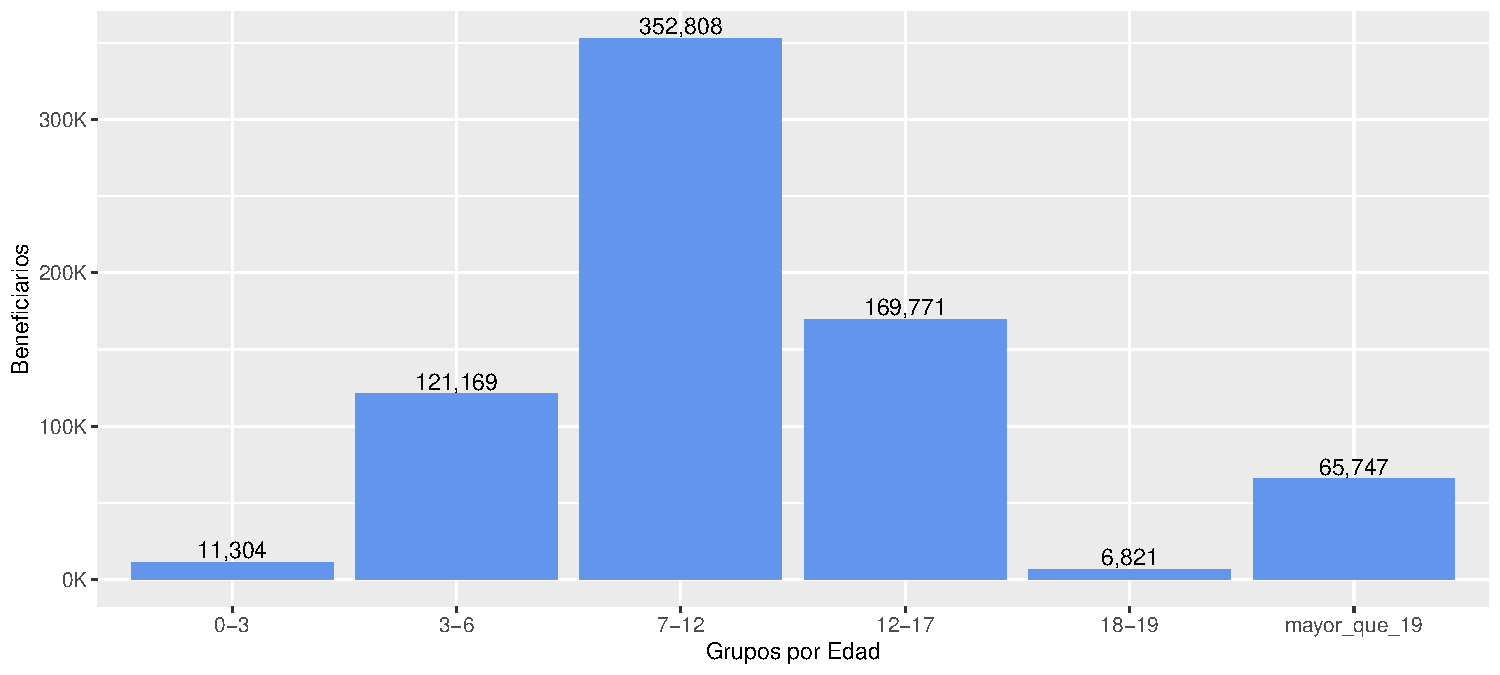
\includegraphics{demo_report_files/figure-latex/beneficiaries by age PLOT-1.pdf}

\hypertarget{beneficiaries-by-age-compared-to-2017-enrollment} of
schoolgoing children aged 3-17 nationwide. Children aged 3-17 consitute
\textbf{88\%} of all UNICEF beneficiaries.
\end{quote}

\begin{longtable}[]{@{}cccc@{}}
\toprule
Edad grupo & beneficiarios & matricula2017 & percent\_total \\
\midrule
\endhead
3-6 & 121,169 & 1,438,475 & 8.423 \\
7-12 & 352,808 & 3,252,505 & 10.85 \\
12-17 & 169,771 & 2,205,724 & 7.697 \\
\bottomrule
\end{longtable}

\hypertarget{changes-since-previous-month}{%
\section{Changes since previous
month}\label{changes-since-previous-month}}

\begin{quote}
The number of individuals reached has increased by \textbf{175,005} in
the past month, reaching a total of \textbf{728,408}. The number of
beneficiary frequencies reached has increased by \textbf{222,618} in the
same period, reaching a total of \textbf{1,071,598}.
\end{quote}

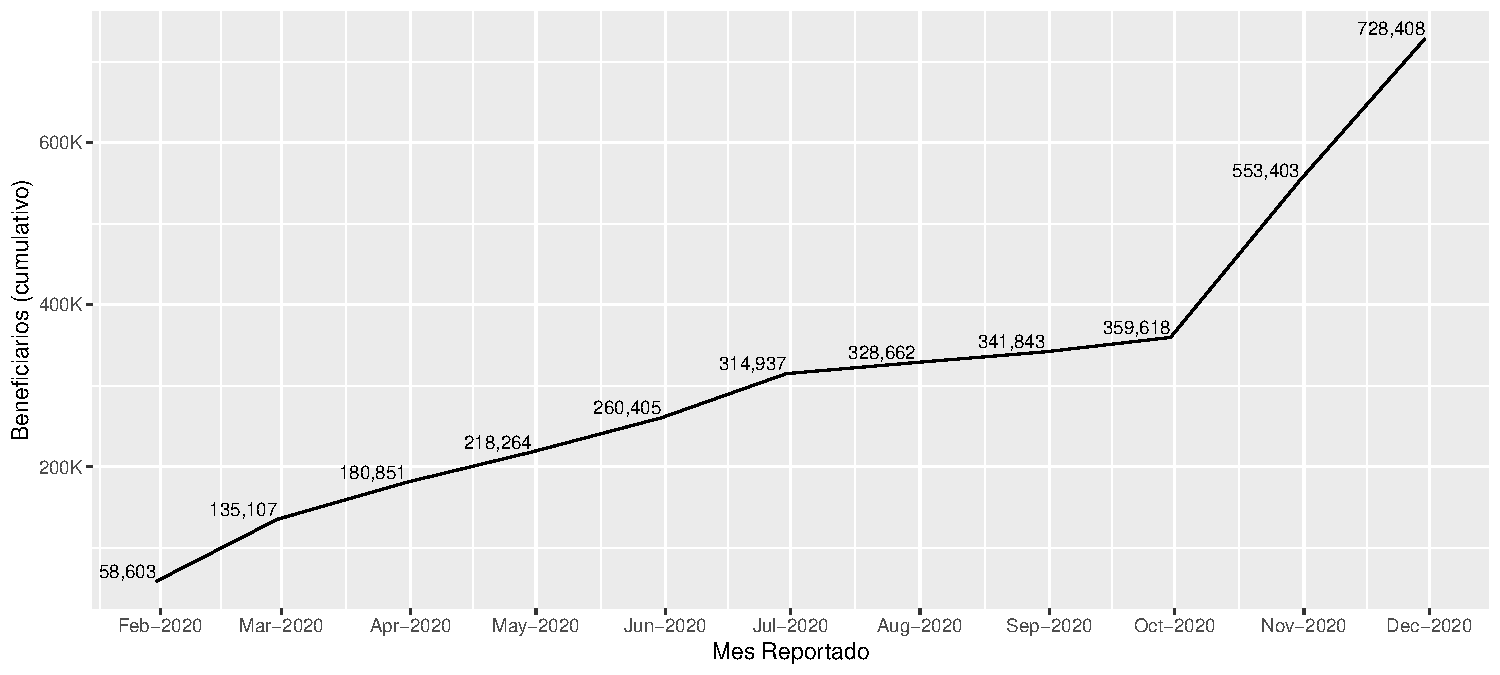
\includegraphics{demo_report_files/figure-latex/cumulative beneficiaries line PLOT-1.pdf}

\hypertarget{progress-by-activity-by-month}{%
\subsection{Progress by activity by
month}\label{progress-by-activity-by-month}}

\emph{mouse over to see details}

\begin{quote}
Progress in recent months has largely been due to the distribution of
education kits and distance learning.
\end{quote}

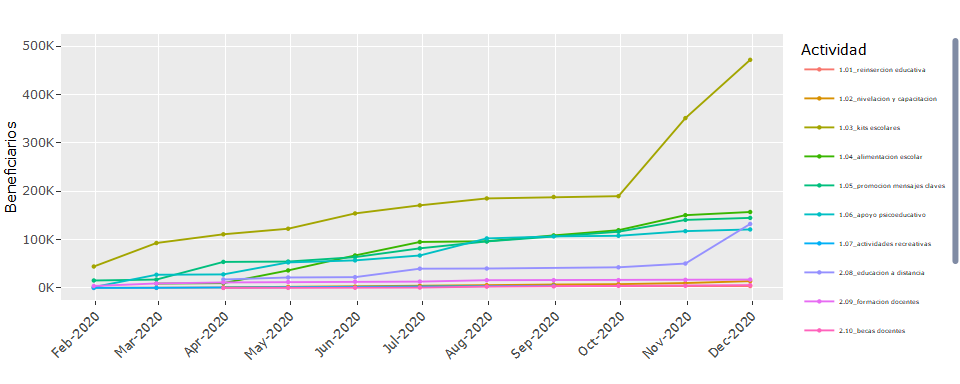
\includegraphics{demo_report_files/figure-latex/line PLOT progress by activity-1.pdf}

\hypertarget{summaries-by-geography}{%
\section{Summaries by geography}\label{summaries-by-geography}}

\hypertarget{beneficiaries-by-state}{%
\subsection{Beneficiaries by state}\label{beneficiaries-by-state}}

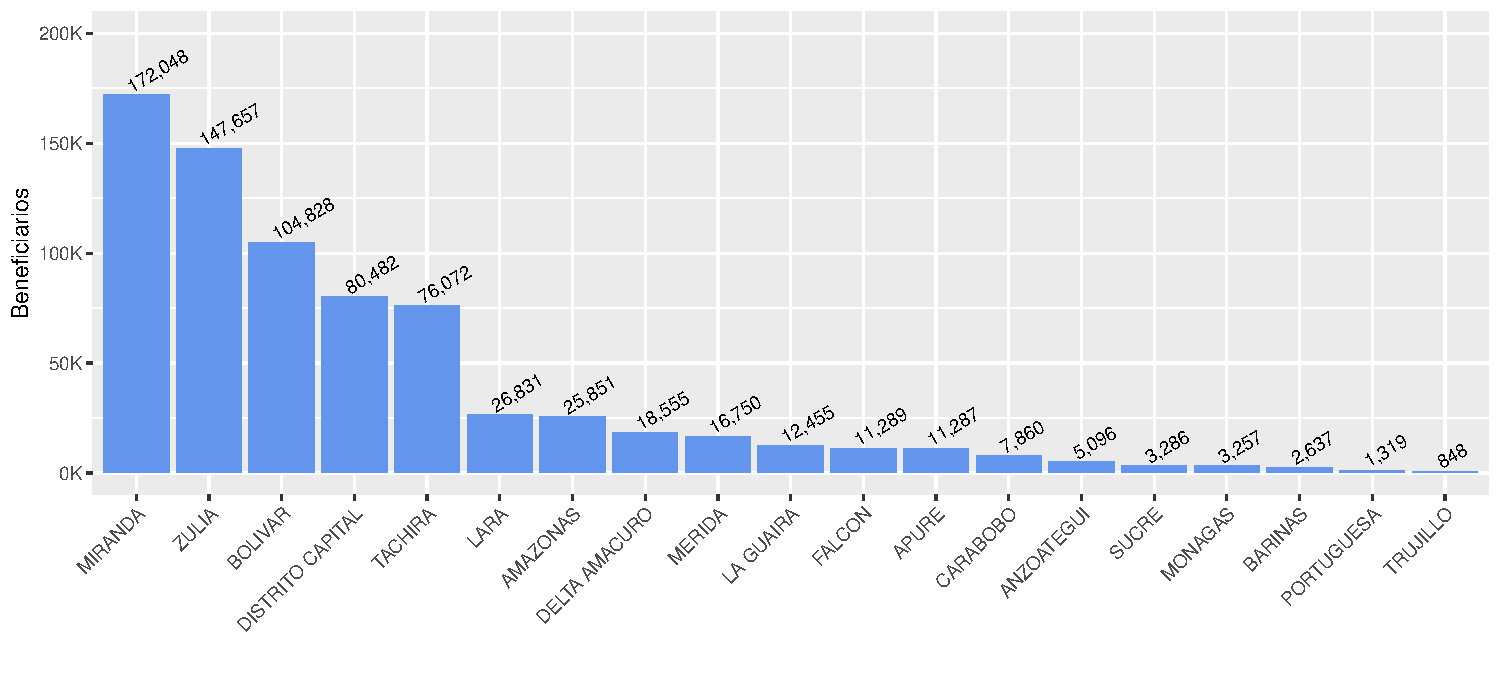
\includegraphics{demo_report_files/figure-latex/unnamed-chunk-1-1.pdf}

\hypertarget{number-of-schools-by-state} are from Miranda and Zulia alone.
\end{quote}

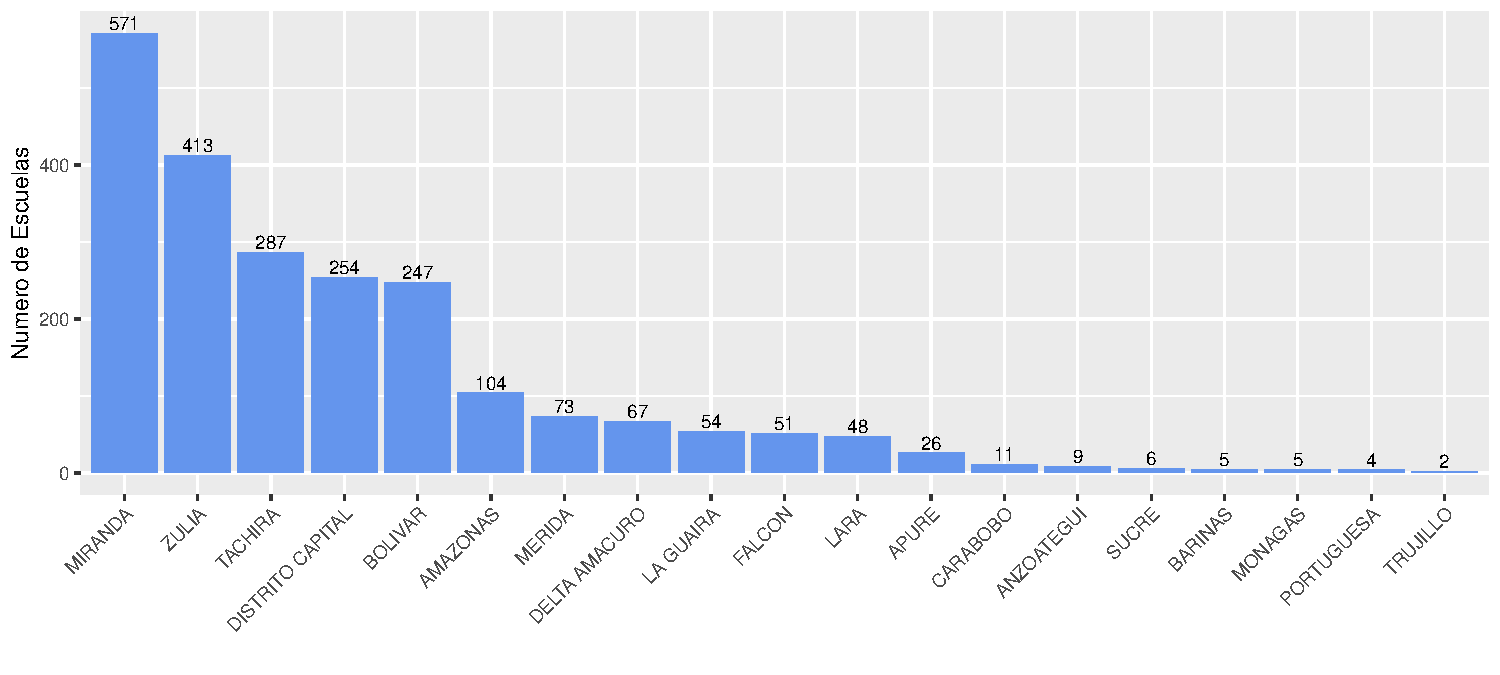
\includegraphics{demo_report_files/figure-latex/PLOT of ubicacion by state-1.pdf}

\hypertarget{scatterplot-of-municipalities}{%
\subsection{Scatterplot of
Municipalities}\label{scatterplot-of-municipalities}}

\emph{logarithmic scale; larger points indicate more beneficiaries
reached, darker blues indicate more activity types}

\emph{mouse over municipalities to see beneficiaries and distinct
activities}

\begin{quote}
A total of \textbf{110} municipalities were reached by the UNICEF
Education programme.
\end{quote}

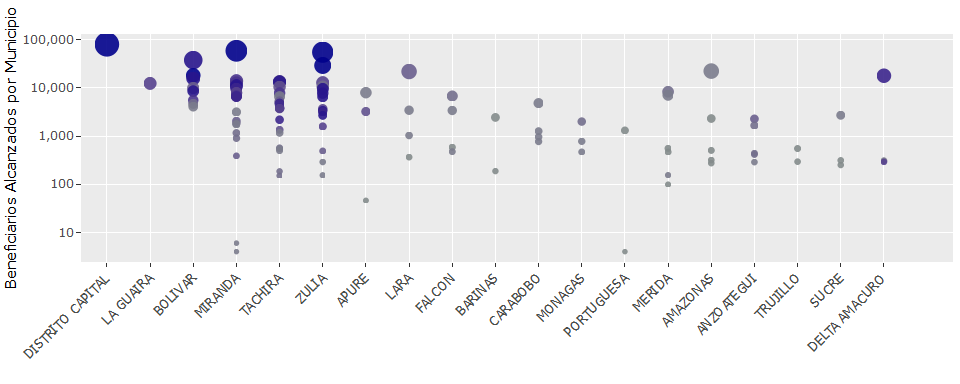
\includegraphics{demo_report_files/figure-latex/scatterPLOT of municipalities by state-1.pdf}

\hypertarget{top-10-municipalities-by-reach-and-coverage}{%
\subsection{Top 10 municipalities by reach and
coverage}\label{top-10-municipalities-by-reach-and-coverage}}

\begin{wraptable}{l}{0pt}

\caption{\label{tab:municipalities top TABLE}by beneficiaries}
\centering
\begin{tabular}[t]{l|l|r}
\hline
estado & municipio & beneficiarios\\
\hline
DISTRITO CAPITAL & LIBERTADOR & 80482\\
\hline
MIRANDA & SUCRE & 59176\\
\hline
ZULIA & MARACAIBO & 55370\\
\hline
BOLIVAR & CARONI & 37908\\
\hline
ZULIA & SAN FRANCISCO & 29369\\
\hline
AMAZONAS & ATURES & 22430\\
\hline
LARA & IRIBARREN & 21977\\
\hline
BOLIVAR & HERES & 18293\\
\hline
DELTA AMACURO & TUCUPITA & 17953\\
\hline
BOLIVAR & CEDENO & 15681\\
\hline
\end{tabular}
\end{wraptable}

\begin{table}

\caption{\label{tab:municipalities top TABLE}by coverage}
\begin{tabular}[t]{l|l|r}
\hline
estado & municipio & coverage\_percent\\
\hline
TACHIRA & FERNANDEZ FEO & 87\\
\hline
TACHIRA & AYACUCHO & 79\\
\hline
ZULIA & MACHIQUES DE PERIJA & 79\\
\hline
AMAZONAS & AUTONOMO AUTANA & 76\\
\hline
TACHIRA & SAMUEL DARIO MALDONADO & 75\\
\hline
TACHIRA & PANAMERICANO & 72\\
\hline
MIRANDA & PLAZA & 68\\
\hline
TACHIRA & INDEPENDENCIA & 68\\
\hline
TACHIRA & JUNIN & 65\\
\hline
MIRANDA & EL HATILLO & 64\\
\hline
\end{tabular}
\end{table}

\begin{quote}
Together, the 10 municipalities with the highest reach (above left) form
\textbf{49\%} of the \textbf{728,400} beneficiaries reached. The average
coverage of the school-age population in the municipalities where UNICEF
is present is \textbf{20\%}. Coverage refers to the percentage of
enrolled children (aged 3-17 years) reached by UNICEF.
\end{quote}

~

\hypertarget{histogram-of-coverage}{%
\subsection{Histogram of Coverage}\label{histogram-of-coverage}}

\begin{quote}
Below is a histogram of munciipalities where UNICEF is present showing
the coverage of enrolled children (aged 3-17). Of note, we have reached
10\% or less of the population in \textbf{55} out of the \textbf{110} in
which we operate. This is in addition to the \textbf{226} where no
UNICEF Education activities have occurred.
\end{quote}

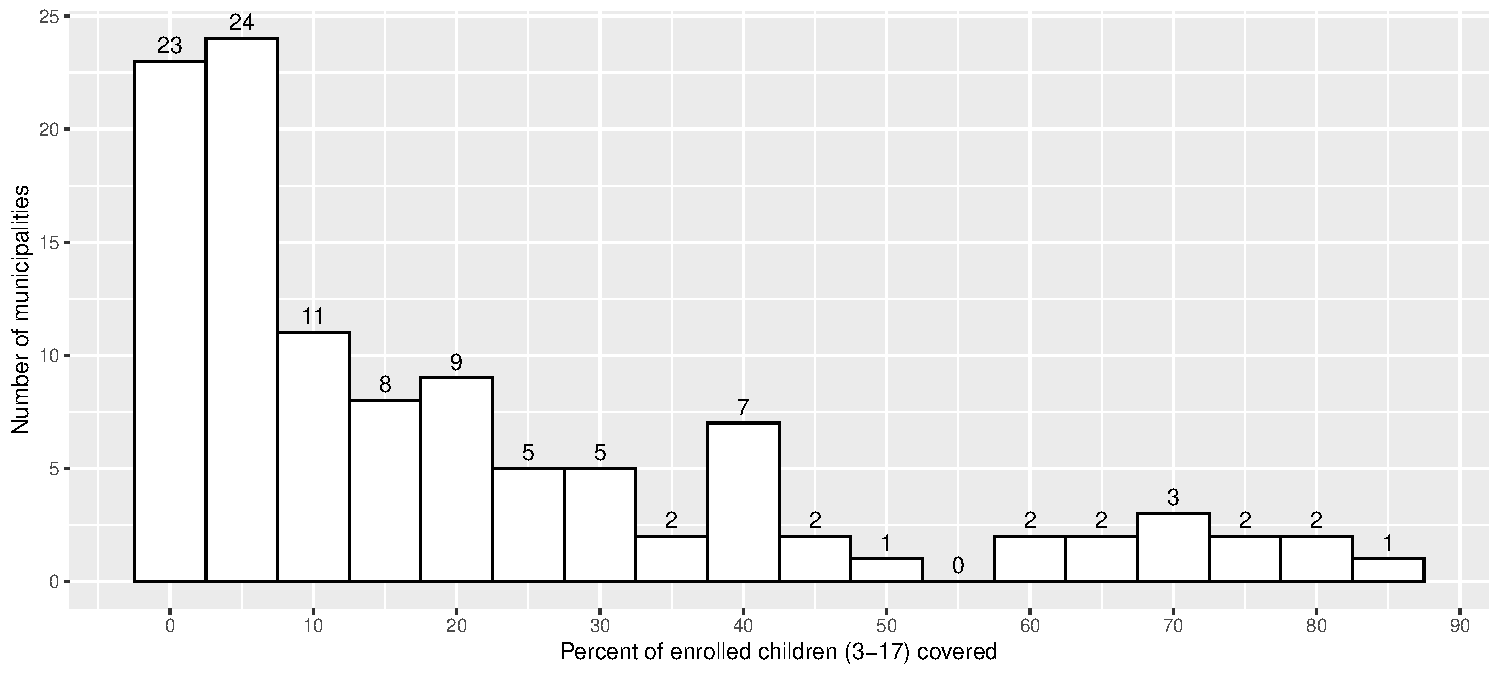
\includegraphics{demo_report_files/figure-latex/PLOT histogram of coverage-1.pdf}

~ ~

\hypertarget{reports-about-partners}{%
\section{Reports about Partners}\label{reports-about-partners}}

\hypertarget{summary-by-partner}{%
\subsection{Summary by Partner}\label{summary-by-partner}}

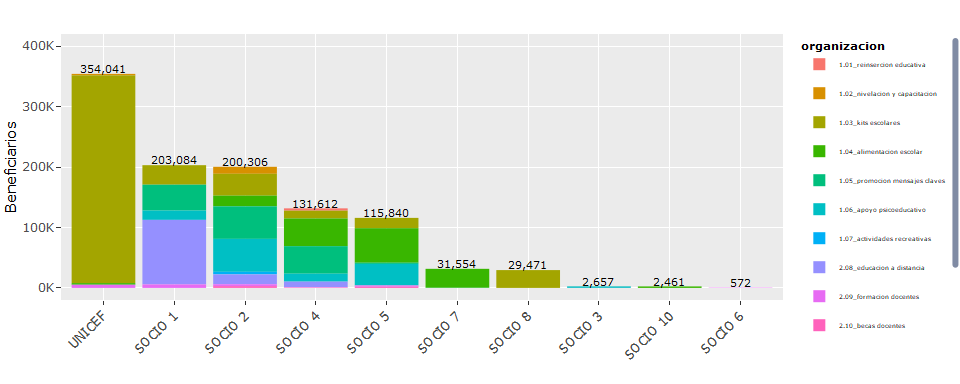
\includegraphics{demo_report_files/figure-latex/PLOT stacked bar partner-1.pdf}

\hypertarget{number-of-different-activities-implemented-by-each-partner}{%
\subsection{Number of different activities implemented by each
partner}\label{number-of-different-activities-implemented-by-each-partner}}

\begin{longtable}[]{@{}
  >{\centering\arraybackslash}p{(\columnwidth - 20\tabcolsep) * \real{0.17}}
  >{\centering\arraybackslash}p{(\columnwidth - 20\tabcolsep) * \real{0.08}}
  >{\centering\arraybackslash}p{(\columnwidth - 20\tabcolsep) * \real{0.08}}
  >{\centering\arraybackslash}p{(\columnwidth - 20\tabcolsep) * \real{0.08}}
  >{\centering\arraybackslash}p{(\columnwidth - 20\tabcolsep) * \real{0.08}}
  >{\centering\arraybackslash}p{(\columnwidth - 20\tabcolsep) * \real{0.07}}
  >{\centering\arraybackslash}p{(\columnwidth - 20\tabcolsep) * \real{0.08}}
  >{\centering\arraybackslash}p{(\columnwidth - 20\tabcolsep) * \real{0.08}}
  >{\centering\arraybackslash}p{(\columnwidth - 20\tabcolsep) * \real{0.08}}
  >{\centering\arraybackslash}p{(\columnwidth - 20\tabcolsep) * \real{0.09}}
  >{\centering\arraybackslash}p{(\columnwidth - 20\tabcolsep) * \real{0.09}}@{}}
\toprule
\endhead
\textbf{partner} & SOCIO 2 & SOCIO 1 & SOCIO 4 & SOCIO 5 & UNICEF &
SOCIO 3 & SOCIO 6 & SOCIO 7 & SOCIO 10 & SOCIO 8 \\
\textbf{num\_activities} & 9 & 8 & 8 & 6 & 6 & 4 & 2 & 2 & 1 & 1 \\
\bottomrule
\end{longtable}

~

\hypertarget{partners-progress-over-time}{%
\subsection{Partners' progress over
time}\label{partners-progress-over-time}}

\emph{mouse over for details}

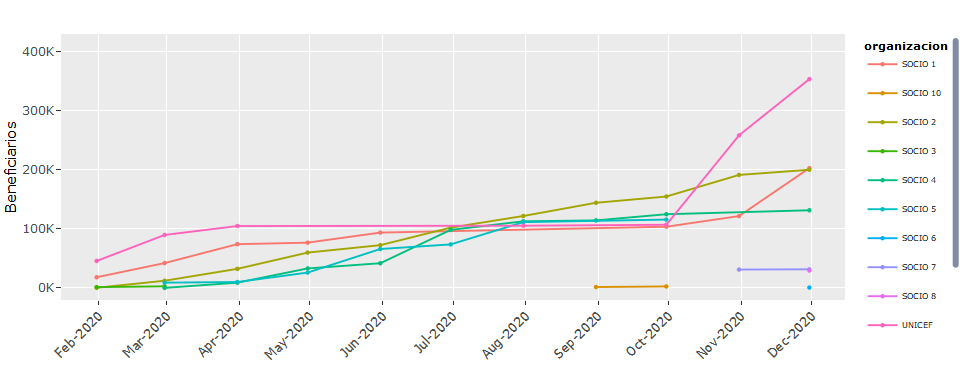
\includegraphics{demo_report_files/figure-latex/line PLOT partners progress-1.pdf}

\hypertarget{summary-table-about-partners-achievements}{%
\subsection{Summary table about partners'
achievements}\label{summary-table-about-partners-achievements}}

\begin{longtable}[]{@{}
  >{\centering\arraybackslash}p{(\columnwidth - 12\tabcolsep) * \real{0.27}}
  >{\centering\arraybackslash}p{(\columnwidth - 12\tabcolsep) * \real{0.14}}
  >{\centering\arraybackslash}p{(\columnwidth - 12\tabcolsep) * \real{0.17}}
  >{\centering\arraybackslash}p{(\columnwidth - 12\tabcolsep) * \real{0.08}}
  >{\centering\arraybackslash}p{(\columnwidth - 12\tabcolsep) * \real{0.08}}
  >{\centering\arraybackslash}p{(\columnwidth - 12\tabcolsep) * \real{0.10}}
  >{\centering\arraybackslash}p{(\columnwidth - 12\tabcolsep) * \real{0.15}}@{}}
\toprule
\begin{minipage}[b]{\linewidth}\centering
organizacion\_implementadora
\end{minipage} & \begin{minipage}[b]{\linewidth}\centering
beneficiarios
\end{minipage} & \begin{minipage}[b]{\linewidth}\centering
percent\_of\_total
\end{minipage} & \begin{minipage}[b]{\linewidth}\centering
male
\end{minipage} & \begin{minipage}[b]{\linewidth}\centering
female
\end{minipage} & \begin{minipage}[b]{\linewidth}\centering
sex\_ratio
\end{minipage} & \begin{minipage}[b]{\linewidth}\centering
municipalities
\end{minipage} \\
\midrule
\endhead
UNICEF & 354,041 & 33.04 & 168,297 & 185,745 & 0.91 & 74 \\
SOCIO 1 & 203,084 & 18.95 & 100,495 & 102,589 & 0.98 & 92 \\
SOCIO 2 & 200,306 & 18.69 & 87,029 & 113,033 & 0.77 & 51 \\
SOCIO 4 & 131,612 & 12.28 & 63,964 & 67,648 & 0.95 & 17 \\
SOCIO 5 & 115,840 & 10.81 & 50,906 & 64,934 & 0.78 & 10 \\
SOCIO 7 & 31,554 & 2.94 & 14,819 & 16,735 & 0.89 & 10 \\
SOCIO 8 & 29,471 & 2.75 & 15,379 & 14,092 & 1.09 & 17 \\
SOCIO 3 & 2,657 & 0.25 & 909 & 1,748 & 0.52 & 3 \\
SOCIO 10 & 2,461 & 0.23 & 1,151 & 1,310 & 0.88 & 1 \\
SOCIO 6 & 572 & 0.05 & 5 & 23 & 0.22 & 7 \\
\bottomrule
\end{longtable}

\hypertarget{maps-and-reference-table}{%
\section{Maps and reference table}\label{maps-and-reference-table}}

\hypertarget{maps-at-municipal-level}{%
\subsection{Maps at municipal level}\label{maps-at-municipal-level}}

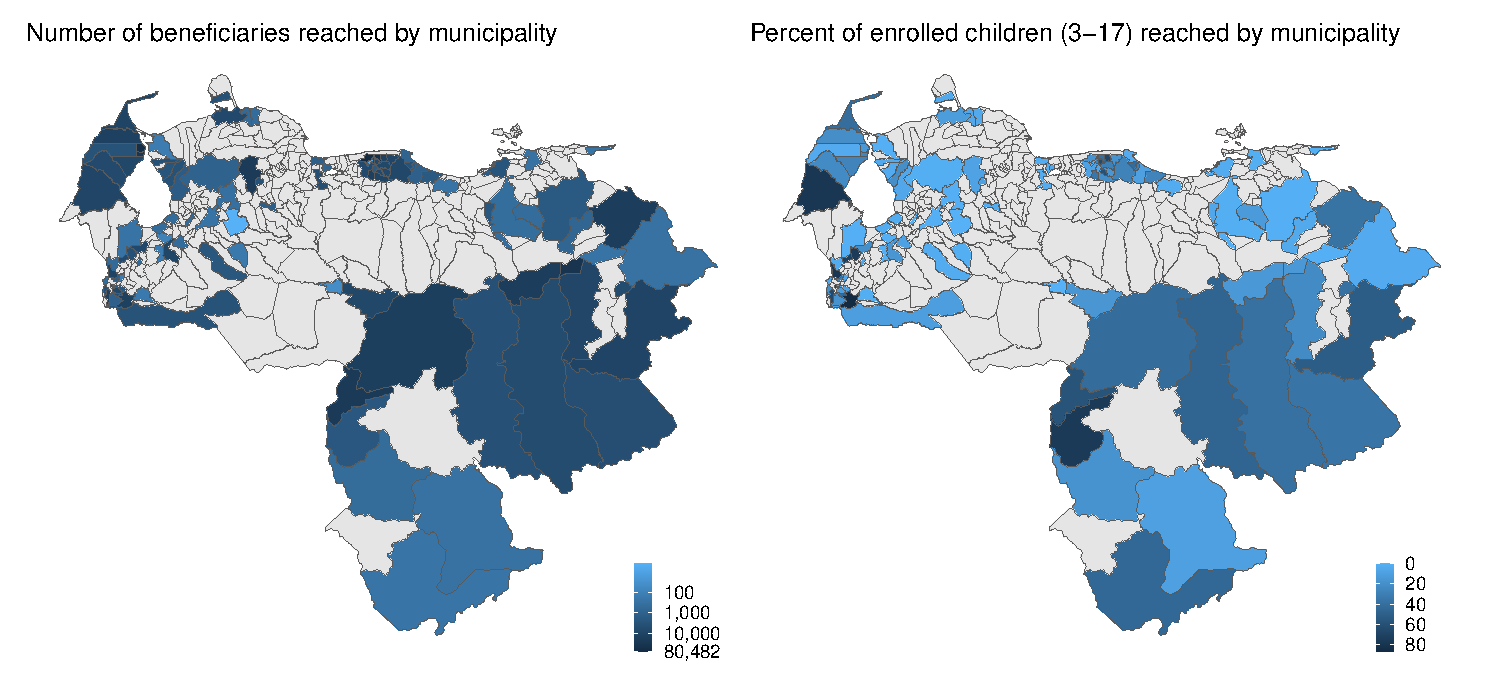
\includegraphics{demo_report_files/figure-latex/MAPS municipal reached and percent reached-1.pdf}

\hypertarget{reference-table---municipal-level}{%
\subsection{Reference table - municipal
level}\label{reference-table---municipal-level}}

\textbf{use \texttt{UNICEF\_present} to filter to municipalities where
the Education programme operates}

\emph{CA01.05 Promocion de mensajes claves para la comunidad escolar is
not included}

\begin{verbatim}
## # A tibble: 335 x 11
##    UNICEF_present estado  municipio beneficiarios beneficiarios_3~ matricula2017
##    <lgl>          <fct>   <chr>             <dbl>            <dbl>         <dbl>
##  1 TRUE           DISTRI~ LIBERTAD~         80482            68863        387048
##  2 TRUE           MIRANDA SUCRE             59176            49884        122738
##  3 TRUE           ZULIA   MARACAIBO         55370            51225        331587
##  4 TRUE           BOLIVAR CARONI            37908            28600        190469
##  5 TRUE           ZULIA   SAN FRAN~         29369            27561        104307
##  6 TRUE           AMAZON~ ATURES            22430            22377         38392
##  7 TRUE           LARA    IRIBARREN         21977            21361        257907
##  8 TRUE           BOLIVAR HERES             18293            13664         89302
##  9 TRUE           DELTA ~ TUCUPITA          17953            14140         37529
## 10 TRUE           BOLIVAR CEDENO            15681            10050         24118
## # ... with 325 more rows, and 5 more variables: coverage_percent <dbl>,
## #   poverty_incidence <dbl>, no_of_activities <int>, poor_persons <dbl>,
## #   total_pop <dbl>
\end{verbatim}

\end{document}
